%%%%%%%%%%%%%%%%%%%%%%%%%%%%%%%%%%%%%%%%%
% Short Sectioned Assignment
% LaTeX Template
% Version 1.0 (5/5/12)
%
% This template has been downloaded from:
% http://www.LaTeXTemplates.com
%
% Original author:
% Frits Wenneker (http://www.howtotex.com)
%
% License:
% CC BY-NC-SA 3.0 (http://creativecommons.org/licenses/by-nc-sa/3.0/)
%
%%%%%%%%%%%%%%%%%%%%%%%%%%%%%%%%%%%%%%%%%

%----------------------------------------------------------------------------------------
%	PACKAGES AND OTHER DOCUMENT CONFIGURATIONS
%----------------------------------------------------------------------------------------

\documentclass[paper=a4, fontsize=11pt]{scrartcl} % A4 paper and 11pt font size

\usepackage{fourier} % Use the Adobe Utopia font for the document - comment this line to return to the LaTeX default
\usepackage[french]{babel} % English language/hyphenation
\usepackage{amsmath,amsfonts,amsthm} % Math packages

\usepackage{lipsum} % Used for inserting dummy 'Lorem ipsum' text into the template
\usepackage{graphicx}
\usepackage{sectsty} % Allows customizing section commands
\allsectionsfont{\centering \normalfont\scshape} % Make all sections centered, the default font and small caps

\usepackage{fancyhdr} % Custom headers and footers
\pagestyle{fancyplain} % Makes all pages in the document conform to the custom headers and footers
\fancyhead{} % No page header - if you want one, create it in the same way as the footers below
\fancyfoot[L]{} % Empty left footer
\fancyfoot[C]{} % Empty center footer
\fancyfoot[R]{\thepage} % Page numbering for right footer
\renewcommand{\headrulewidth}{0pt} % Remove header underlines
\renewcommand{\footrulewidth}{0pt} % Remove footer underlines
\setlength{\headheight}{13.6pt} % Customize the height of the header

\numberwithin{equation}{section} % Number equations within sections (i.e. 1.1, 1.2, 2.1, 2.2 instead of 1, 2, 3, 4)
\numberwithin{figure}{section} % Number figures within sections (i.e. 1.1, 1.2, 2.1, 2.2 instead of 1, 2, 3, 4)
\numberwithin{table}{section} % Number tables within sections (i.e. 1.1, 1.2, 2.1, 2.2 instead of 1, 2, 3, 4)

\setlength\parindent{0pt} % Removes all indentation from paragraphs - comment this line for an assignment with lots of text

%----------------------------------------------------------------------------------------
%	TITLE SECTION
%----------------------------------------------------------------------------------------

\newcommand{\horrule}[1]{\rule{\linewidth}{#1}} % Create horizontal rule command with 1 argument of height

\title{	
\normalfont \normalsize 
\textsc{Ecole Centrale de Nantes} \\ [25pt] % Your university, school and/or department name(s)
\horrule{0.5pt} \\[0.4cm] % Thin top horizontal rule
\huge Option Informatique - TD MADIS \\ % The assignment title
\horrule{2pt} \\[0.5cm] % Thick bottom horizontal rule
}

%\author{Durée 1h - Aucun document autorisé} % Your name

%\date{\normalsize\today} % Today's date or a custom date

\begin{document}

\maketitle % Print the title

\section{L'itinéraire de Michel Strogoff}

Partant de Moscou, Michel Strogoff, courrier du tsar, devait rejoindre Irkoutsk. Avant de partir, il avait consulté une voyante qui lui avait dit entre autres choses : 
"Après Kaza, méfiez-vous du ciel, à Omsk attention aux Tartares, dans Tomsk attention aux yeux, après Tomsk méfiez-vous de l'eau, et, surtout prenez garde partout à un grand brun avec des bottes noires". Strogoff avait alors reporté sur une carte pour chaque liaison entre deux villes les "chances" de réussite ; ces chances étaient exprimées par un nombre entre un et dix (mesurant le nombre de chances sur dix de succès). Ignorant le calcul des probabilités, il avait alors choisi son itinéraire en maximisant la somme des chances...

Pour simplifier, les villes ont été numérotées et les itinéraires possibles sont représentés sur le graphe de la figure~\ref{fig:ms}.

\begin{enumerate}
\item Déterminer l'itinéraire de Michel Strogoff
\item Quelle était alors sous l'hypothèse d'indépendance des variables aléatoires "chances de succès", la probabilité pour que Strogoff réussisse ?
\item Quel aurait été son itinéraire s'il avait connu les principes du calcul des probabilités ?
\end{enumerate}

\begin{figure}[htbp]
\begin{center}
	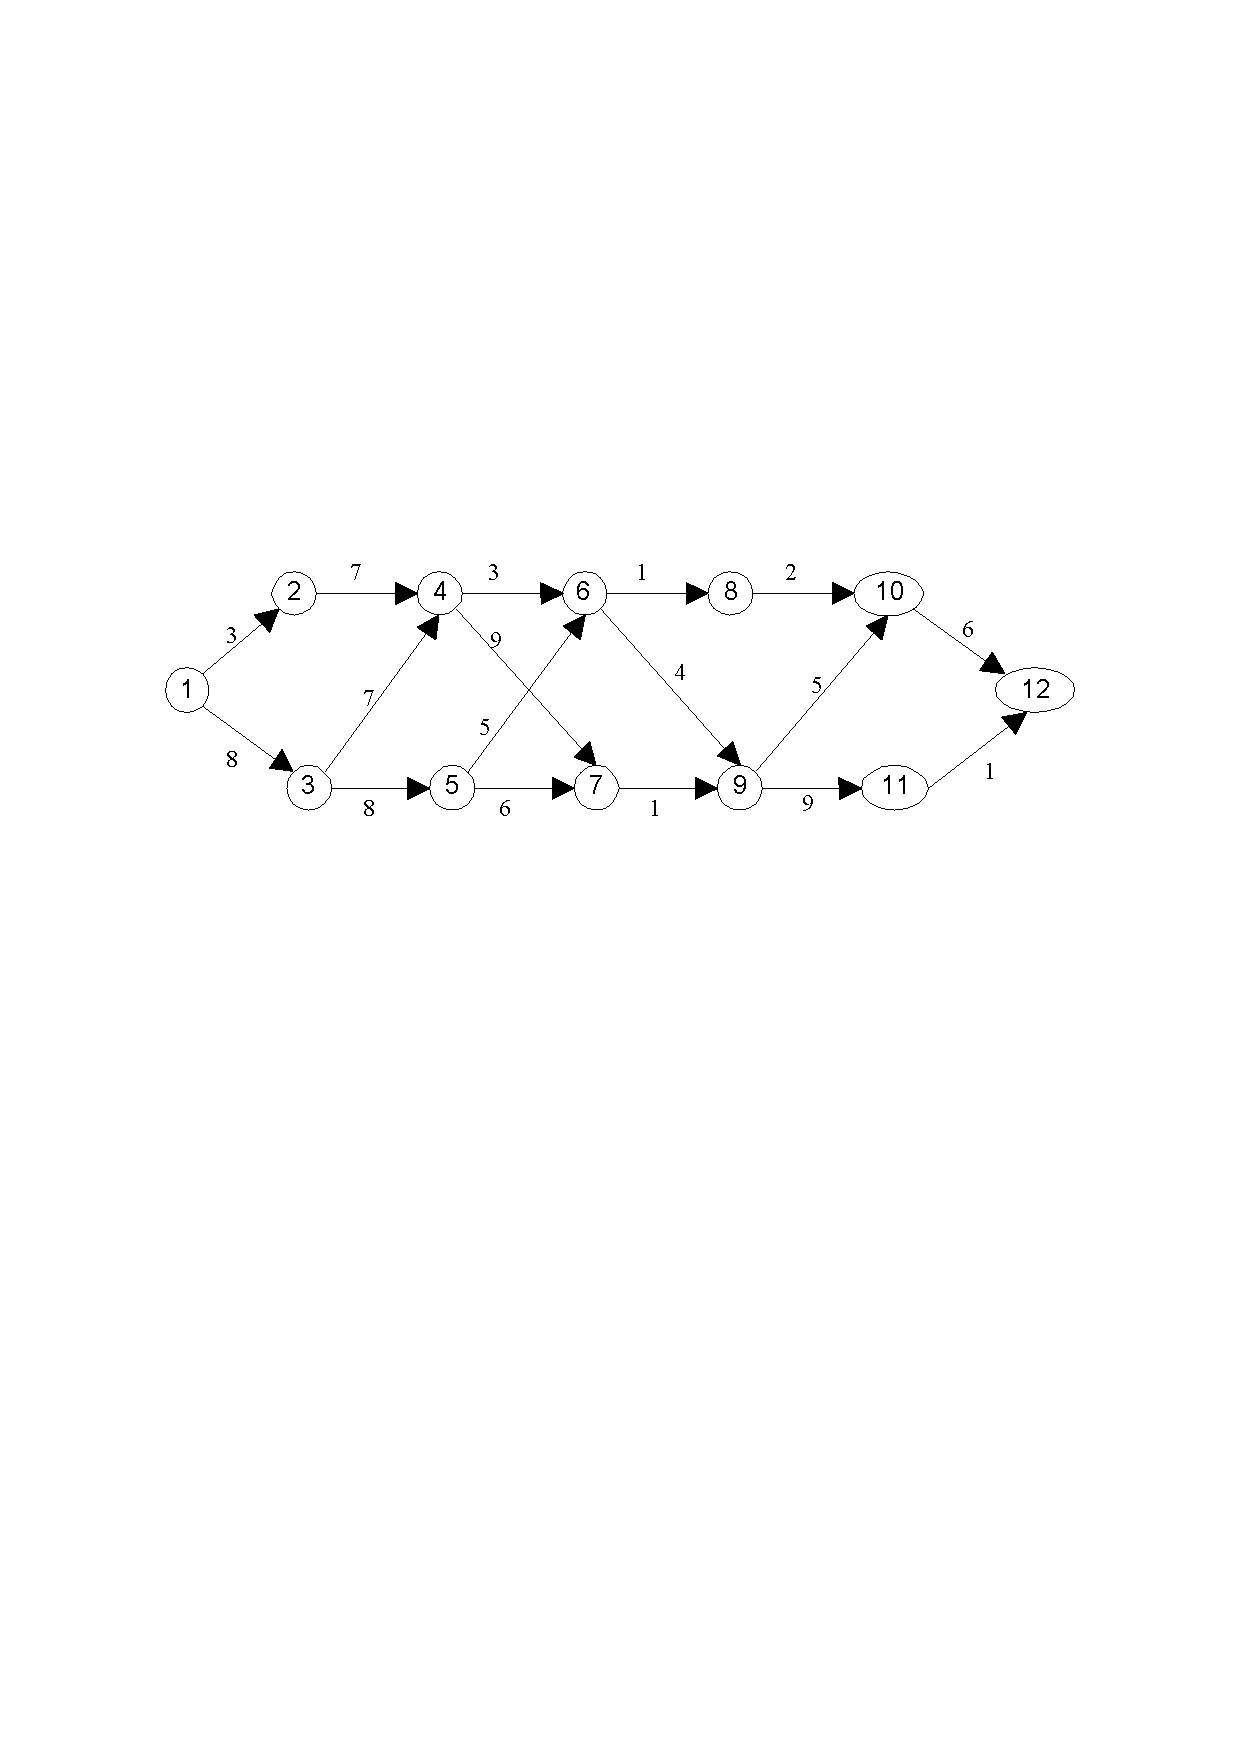
\includegraphics[width=.8\textwidth]{strogoff.pdf}
	\caption{Itinéraires possible et chances de succès pour un trajet d'une ville à l'autre}
	\label{fig:ms}
\end{center}
\end{figure}

\section{Débit réseau}

On s'intéresse maintenant à un problème de réseau. Pour une visio-conférence, on doit envoyer des paquets de données d'un point A vers un point B. TCP/IP permettant un routage des paquets, les paquets de données peuvent circuler sur différentes connexions avec un débit différent. On fera l'hypothèse que les paquets arrivent en ordre. 

\begin{figure}[htbp]
\begin{center}
	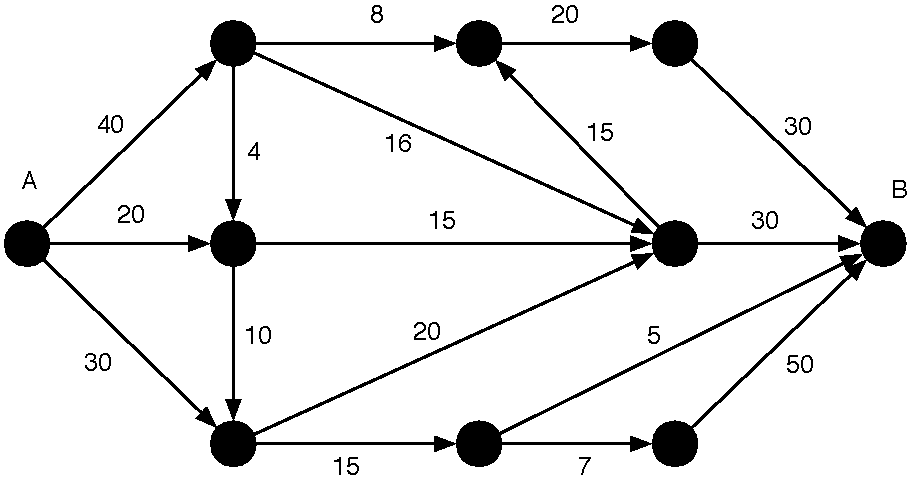
\includegraphics[width=.8\textwidth]{graphe1.pdf}
\end{center}
\end{figure}

\begin{enumerate}
\item Calculer le débit maximum atteignable avec le réseau de la figure précédente.
\item Quelle est la première liaison dont il faut augmenter le débit pour augmenter le débit global ?
\end{enumerate}
\section{Acheminement de passagers}

Lors de la mise en place d'un voyage organisé, un vol charter est
prévu au départ d'une ville F, un samedi soir. Les participants à ce
vol viennent de trois villes A, B et C avec des possibilités limitées
d'acheminement de ces villes jusqu'à F. Des départs sont prévus au
départ de A, B et C les jeudi, vendredi et samedi matins. Les
destinations possibles et le nombre de places disponibles sont
indiquées dans le tableau~\ref{tab:vol}.

\begin{table}[htbp]
  \begin{center}
    \begin{tabular}{|l|ccccc|}
      \hline
      & A vers B & A vers F & B vers C & B vers F & C vers F \\
     \hline 
      jeudi matin & 10 & 20 & 30 & 30 & 20 \\
      vendredi matin & 10 & 20 & 30 & 20 & 20 \\
      samedi matin & 0 & 25 & 0 & 65 & 40 \\
      \hline
    \end{tabular}
    \caption{Capacités de transport}
    \label{tab:vol}
  \end{center}
\end{table}

Pour chacun des départs, l'arrivée a lieu le soir même. Il est
possible de prévoir des transits et de passer une ou plusieurs nuits
dans chacune des villes, en fonction des capacités d'hébergement
répertoriées dans le tableau~\ref{tab:nuit}.

\begin{table}[htbp]
  \begin{center}
    \begin{tabular}{|l|cccc|}
      \hline
      & A & B & C & F \\
      \hline
      nuit de jeudi à vendredi & 30 & 50 & 40 & 25 \\
      nuit de vendredi à samedi & 15 & 55 & 40 & 40 \\
      \hline
    \end{tabular}
    \caption{Capacités d'accueil}
    \label{tab:nuit}
  \end{center}
\end{table}

Le nombre de personnes pouvant rester dans une ville durant la journée
n'est pas limité. Tous les participants du voyage doivent être pris en
charge à partir du jeudi matin (transport et hébergement). Il y a une
limitation a priori sur le nombre d'inscriptions (100 participants au
départ de A, autant de B et C). 

On cherche à acheminer le plus de participants possibles pour le vol
charter en tenant compte de ces contraintes.

\begin{enumerate}
\item définir un réseau de transport avec capacités permettant de
   formaliser le problème comme un problème de flot
   maximal. (indication : pour chaque ville $\alpha$, considérer deux
   sommets $\alpha_i$ et $\alpha_i'$ correspondant respectivement au
   matin et au soir du jour $j$).

\item résoudre le problème. combien de participants issus de A
   (respectivement B et C) pourront bénéficier du vol charter, selon
   la solution trouvée ?
\end{enumerate}

\section{Grossiste en fleurs}

Un grossiste en fleurs assure le transport depuis Marseille et Valence vers Paris. Ce transport est effectué par camionnette de Valence à Carpentras et de Marseille à Carpentras ou Grenoble, puis par train ou avion de Carpentras à Paris et par train de Grenoble à Paris. On désire étudier le transport global par semaine de façon à envoyer un maximum de fleurs à Paris à coût minimal bien entendu.

Les camionnettes disponibles à Valence permettent d'acheminer au plus 400 cartons par semaine vers Carpentras au coût unitaire de 2 ; celles de Marseille 400 cartons dont la moitié vers Carpentras au coût unitaire de 3 et l'autre moitié vers Grenoble au coût de 2. De plus, on doit limiter le transport par le train à 300 cartons dont 200 au plus depuis Carpentras, le coût unitaire étant alors de 10 depuis Grenoble et de 9 depuis Carpentras. Par avion, le coût unitaire est de 16. 

La production de Marseille ne peut dépasser 200 cartons, celle de Valence est toujours excédentaire.

\begin{enumerate}
\item Modéliser le problème sous forme de graphe 
\item Après avoir simplifié au maximum le graphe, résoudre le problème à l'aide de l'algorithme de Roy.

\end{enumerate}

\end{document}
%%% Local Variables: 
%%% mode: latex
%%% TeX-master: t
%%% End: 
